\documentclass[svgnames,11pt]{beamer}
\input{/home/tof/Documents/Cozy/latex-include/preambule_commun.tex}
\input{/home/tof/Documents/Cozy/latex-include/preambule_beamer.tex}
\usepackage{pgfpages} \setbeameroption{show notes on second screen=left}
\author[]{Christophe Viroulaud}
\title{Trier des cartes}
\date{}
%\logo{}
\institute{Première - NSI}

\begin{document}
\begin{frame}
\titlepage
\end{frame}


\section{Problématique}
\begin{frame}
    \frametitle{}

    Trier un jeu de cartes est une opération qui trouve des applications en informatique.
    \begin{center}
        \framebox{Existe-t-il plusieurs méthodes pour trier des données?}
    \end{center}

\end{frame}

\section{Trier des cartes manuellement}
\begin{frame}
    \frametitle{}

    \begin{center}
        \centering
        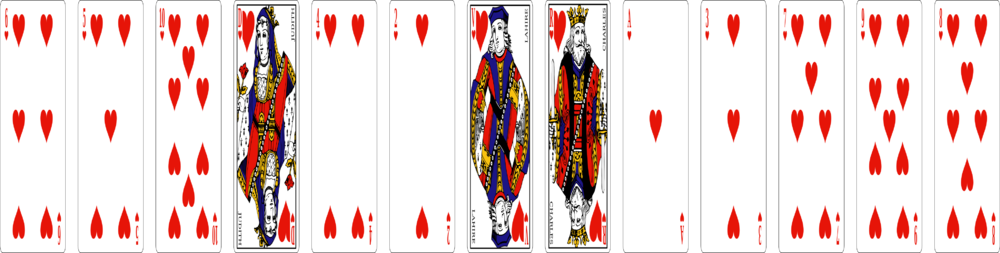
\includegraphics[width=10cm]{ressources/jeu-coeur-melange.png}
        \captionof{figure}{Cartes mélangées}
        \label{pique}
    \end{center}

\end{frame}

\begin{frame}
    \frametitle{}
    \begin{activite}
        \begin{enumerate}
            \item Prendre le paquet de cartes mélangées et les étaler sur la table.
            \item Trier les cartes.
            \item Formaliser la méthode utilisée sous forme d'un algorithme.
        \end{enumerate}
    \end{activite}

\end{frame}

\begin{frame}[label=menu]
    \frametitle{\hypertarget{menu}{Différentes méthodes}}

    \begin{itemize}
        \item \hyperlink{selection1}{Tri par sélection en place}
        \item \hyperlink{selection2}{Tri par sélection dans un nouveau tableau}
        \item \hyperlink{insertion1}{Tri par insertion en place}
        \item \hyperlink{insertion2}{Tri par insertion dans un nouveau tableau}
    \end{itemize}

\end{frame}
\begin{frame}[fragile]
    \frametitle{\hypertarget{selection1}{Tri par sélection en place}
    }
    \begin{center}
        \begin{lstlisting}[language=bash, basicstyle=\small]
Pour chaque carte du tas
    Trouver la plus petite carte dans la partie non triée.
    Échanger cette carte avec la première de la partie non triée.
        \end{lstlisting}
        \captionof{code}{Tri par sélection (en place)}
        \label{CODE}
    \end{center}
\hyperlink{menu}{Retour menu}
\end{frame}
\begin{frame}
    \frametitle{Tri par sélection en place}

    \begin{center}
        \centering
        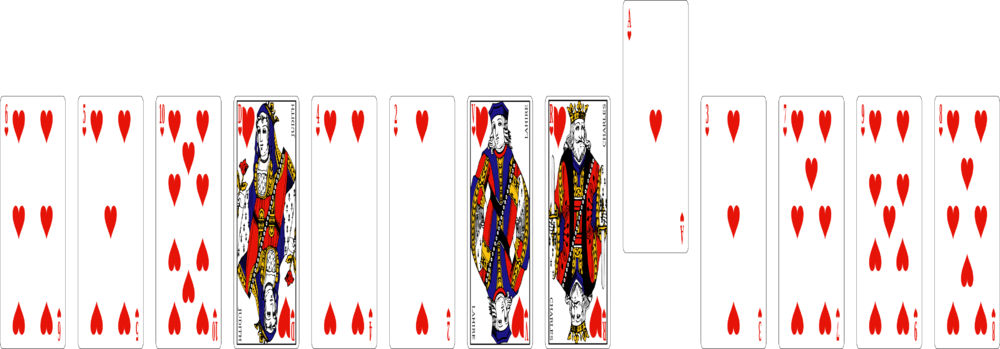
\includegraphics[width=10cm]{ressources/selection-1.png}
        \captionof{figure}{Sélectionne la plus petite du tas non trié}
        \label{pique}
    \end{center}
    \hyperlink{menu}{Retour menu}

\end{frame}

\begin{frame}
    \frametitle{Tri par sélection en place}

    \begin{center}
        \centering
        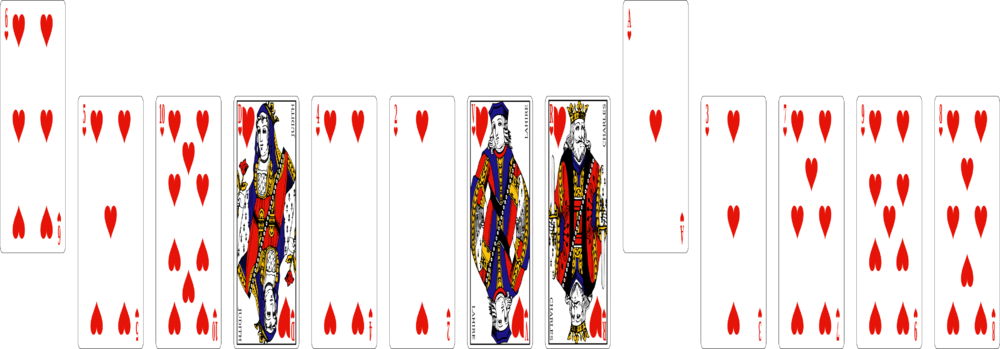
\includegraphics[width=10cm]{ressources/selection-1-2.png}
        \captionof{figure}{Échange avec la première carte du tas non trié}
        \label{pique}
    \end{center}
    \hyperlink{menu}{Retour menu}

\end{frame}

\begin{frame}
    \frametitle{Tri par sélection en place}

    \begin{center}
        \centering
        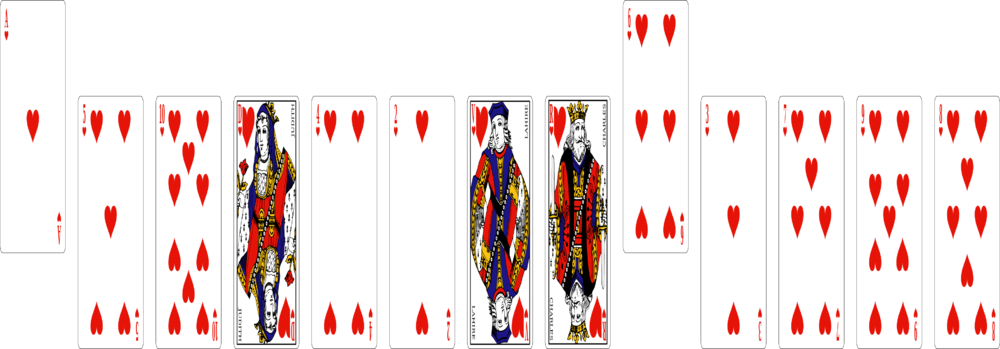
\includegraphics[width=10cm]{ressources/selection-1-3.png}
        \captionof{figure}{Échange avec la première carte du tas non trié}
        \label{pique}
    \end{center}
    \hyperlink{menu}{Retour menu}

\end{frame}

\begin{frame}
    \frametitle{Tri par sélection en place}

    \begin{center}
        \centering
        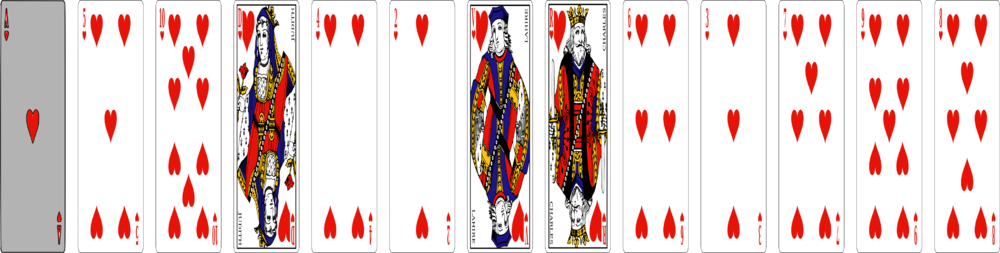
\includegraphics[width=10cm]{ressources/selection-1-4.png}
        \captionof{figure}{La carte est à sa place}
        \label{pique}
    \end{center}
    \hyperlink{menu}{Retour menu}

\end{frame}

\begin{frame}
    \frametitle{Tri par sélection en place}

    \begin{center}
        \centering
        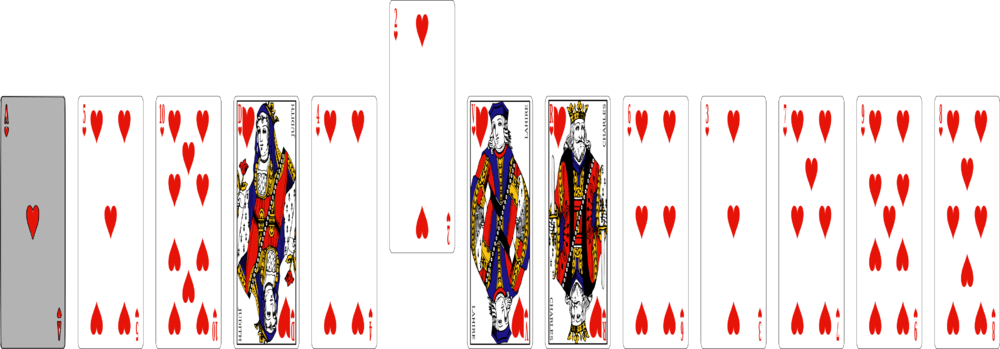
\includegraphics[width=10cm]{ressources/selection-2.png}
        \captionof{figure}{Sélectionne la plus petite du tas non trié}
        \label{pique}
    \end{center}
    \hyperlink{menu}{Retour menu}

\end{frame}

\begin{frame}
    \frametitle{Tri par sélection en place}

    \begin{center}
        \centering
        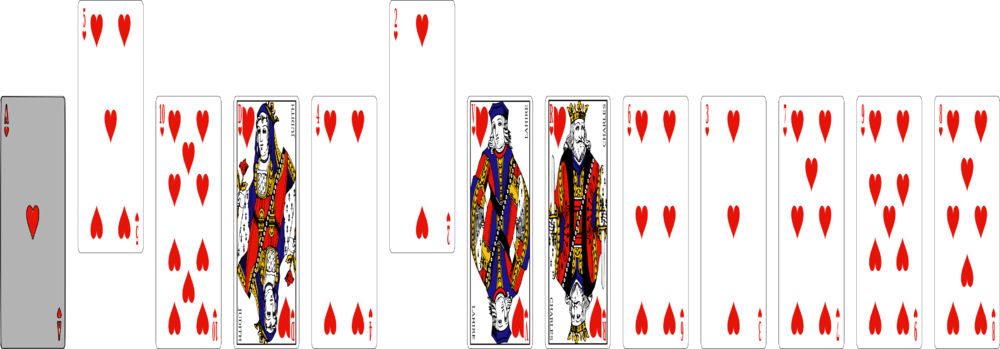
\includegraphics[width=10cm]{ressources/selection-2-2.png}
        \captionof{figure}{Échange avec la première carte du tas non trié}
        \label{pique}
    \end{center}
    \hyperlink{menu}{Retour menu}

\end{frame}

\begin{frame}
    \frametitle{Tri par sélection en place}

    \begin{center}
        \centering
        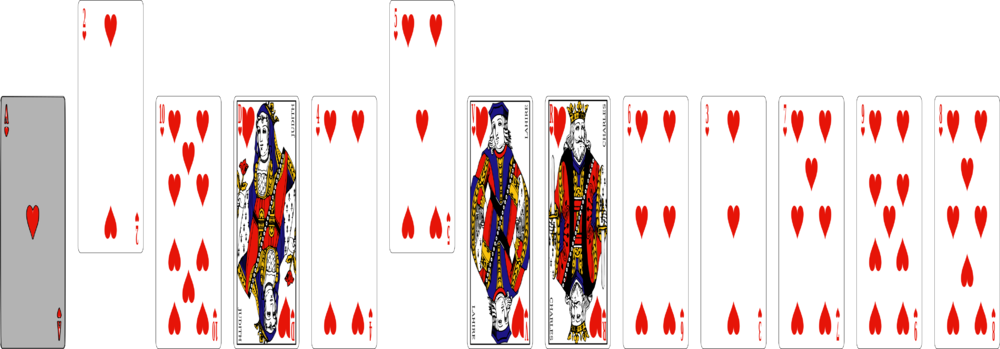
\includegraphics[width=10cm]{ressources/selection-2-3.png}
        \captionof{figure}{Échange avec la première carte du tas non trié}
        \label{pique}
    \end{center}
    \hyperlink{menu}{Retour menu}

\end{frame}

\begin{frame}
    \frametitle{Tri par sélection en place}

    \begin{center}
        \centering
        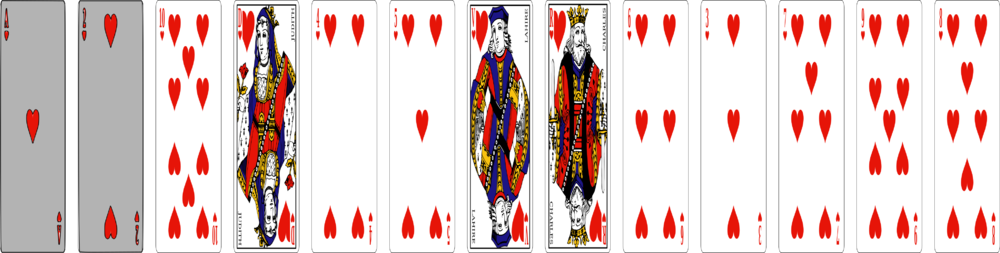
\includegraphics[width=10cm]{ressources/selection-2-4.png}
        \captionof{figure}{La carte est à sa place}
        \label{pique}
    \end{center}
    \hyperlink{menu}{Retour menu}

\end{frame}


\begin{frame}[fragile]
    \frametitle{\hypertarget{selection2}{Tri par sélection - nouveau tableau}
    }
    \begin{center}
        \begin{lstlisting}[language=bash, basicstyle=\small, xrightmargin=1em]
Pour chaque carte du tas
    Trouver la plus petite carte du tableau non trié.
    La placer à la fin du tableau trié.
        \end{lstlisting}
        \captionof{code}{Tri par sélection dans un nouveau tableau}
        \label{CODE}
    \end{center}
\hyperlink{menu}{Retour menu}
\end{frame}
\begin{frame}
    \frametitle{Tri par sélection - nouveau tableau}

    \begin{center}
        \centering
        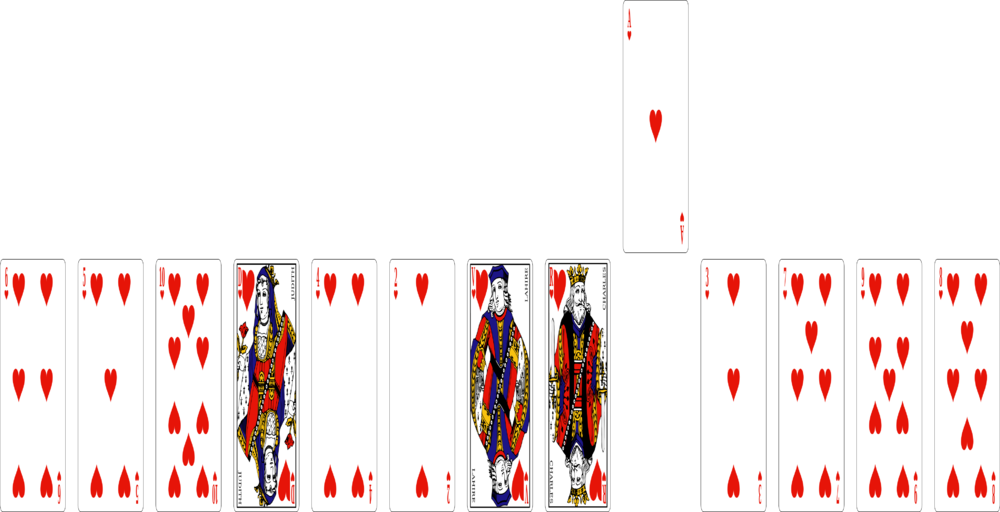
\includegraphics[width=10cm]{ressources/selection2-1.png}
        \captionof{figure}{Trouve la plus petite du tas non trié}
        \label{pique}
    \end{center}
    \hyperlink{menu}{Retour menu}

\end{frame}

\begin{frame}
    \frametitle{Tri par sélection - nouveau tableau}

    \begin{center}
        \centering
        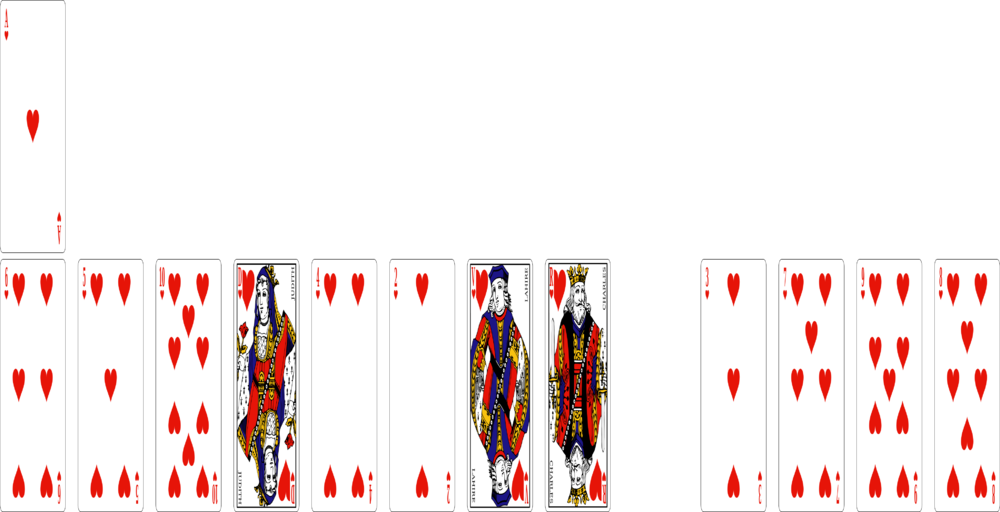
\includegraphics[width=10cm]{ressources/selection2-2.png}
        \captionof{figure}{La place à la fin du tableau trié}
        \label{pique}
    \end{center}
    \hyperlink{menu}{Retour menu}

\end{frame}

\begin{frame}
    \frametitle{Tri par sélection - nouveau tableau}

    \begin{center}
        \centering
        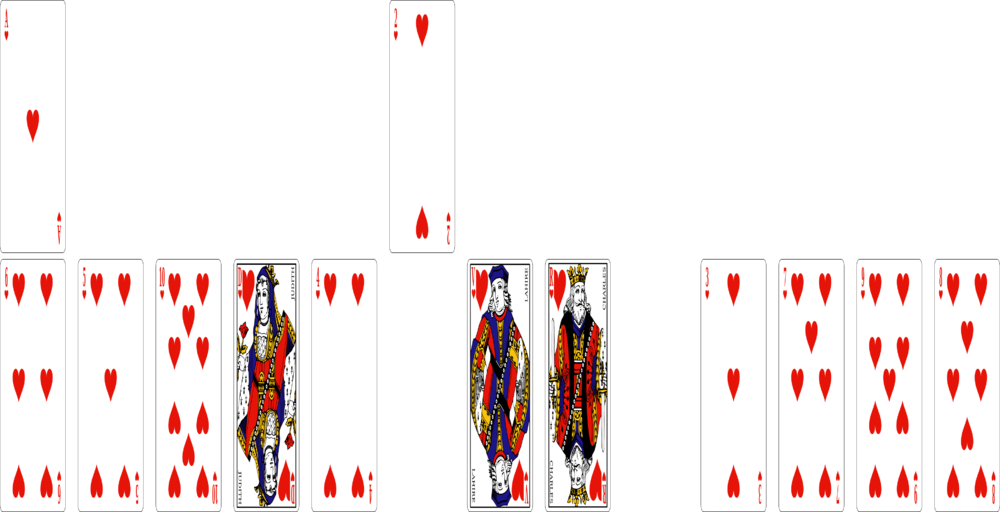
\includegraphics[width=10cm]{ressources/selection2-3.png}
        \captionof{figure}{Trouve la plus petite du tas non trié}
        \label{pique}
    \end{center}
    \hyperlink{menu}{Retour menu}

\end{frame}

\begin{frame}
    \frametitle{Tri par sélection - nouveau tableau}

    \begin{center}
        \centering
        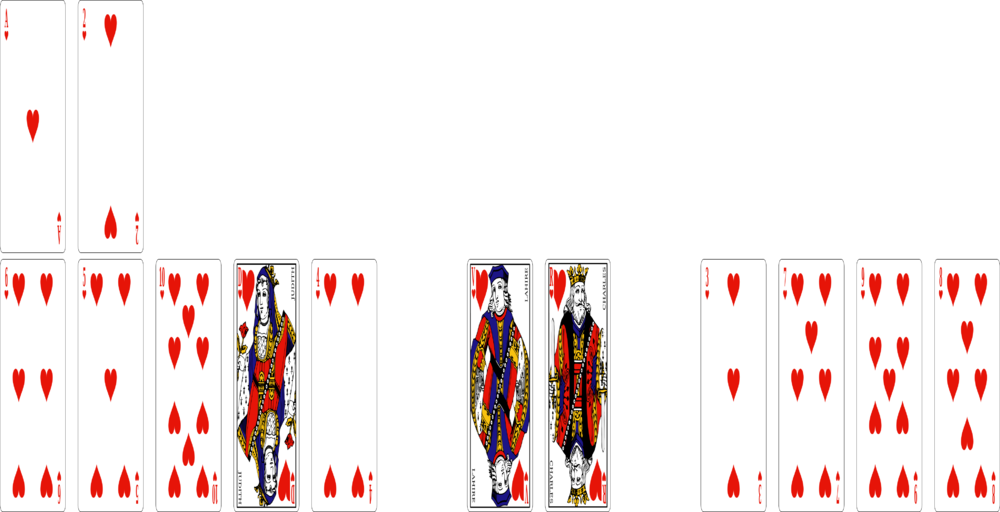
\includegraphics[width=10cm]{ressources/selection2-4.png}
        \captionof{figure}{La place à la fin du tableau trié}
        \label{pique}
    \end{center}
    \hyperlink{menu}{Retour menu}

\end{frame}


\begin{frame}[fragile]
    \frametitle{\hypertarget{insertion1}{Tri par insertion en place}}

    \begin{center}
        \begin{lstlisting}[language=bash, basicstyle=\small, xrightmargin=1em]
Pour chaque carte du tas
    Mémoriser la carte en cours
    Décaler vers la droite toutes les cartes précédentes, supérieures à la carte en cours.
    Insérer la carte en cours dans l'espace vide.
        \end{lstlisting}
        \captionof{code}{Tri par insertion (en place)}
        \label{CODE}
    \end{center}
    \hyperlink{menu}{Retour menu}

\end{frame}

\begin{frame}
    \frametitle{Tri par insertion en place}

    \begin{center}
        \centering
        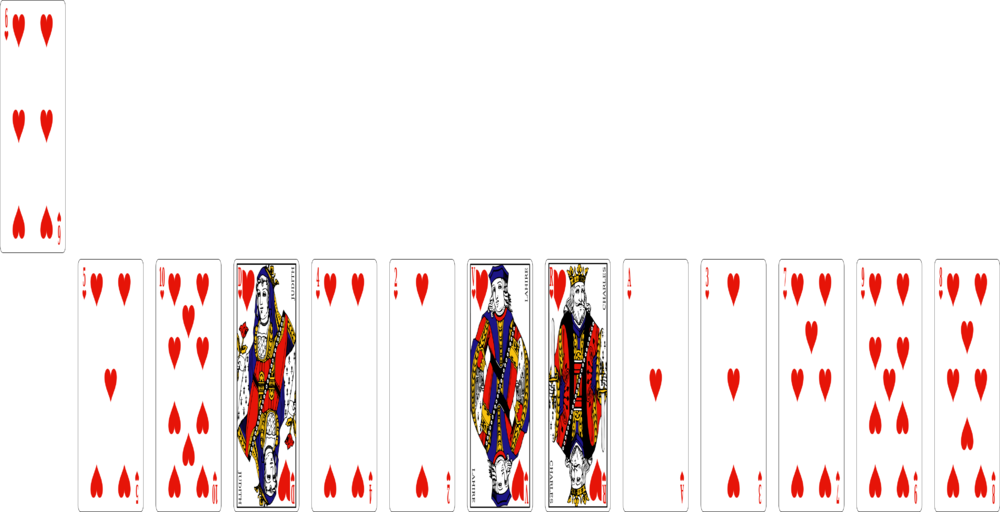
\includegraphics[width=10cm]{ressources/insertion-1.png}
        \captionof{figure}{Mémoriser la première carte dans le tas non trié}
        \label{pique}
    \end{center}
    \hyperlink{menu}{Retour menu}

\end{frame}

\begin{frame}
    \frametitle{Tri par insertion en place}

    \begin{center}
        \centering
        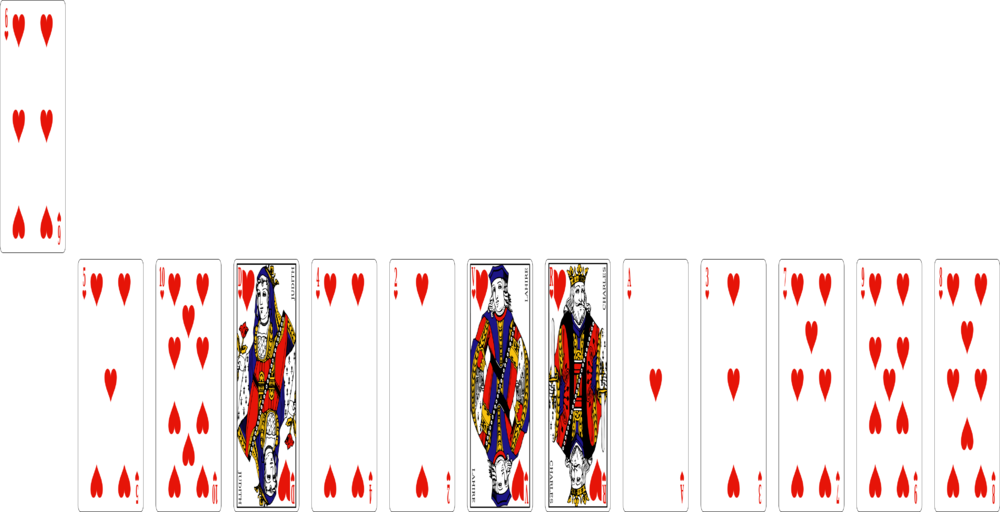
\includegraphics[width=10cm]{ressources/insertion-1.png}
        \captionof{figure}{Décaler les cartes supérieures déjà triées}
        \label{pique}
    \end{center}
    \note{Ici pas de carte triée encore}
    \hyperlink{menu}{Retour menu}

\end{frame}

\begin{frame}
    \frametitle{Tri par insertion en place}

    \begin{center}
        \centering
        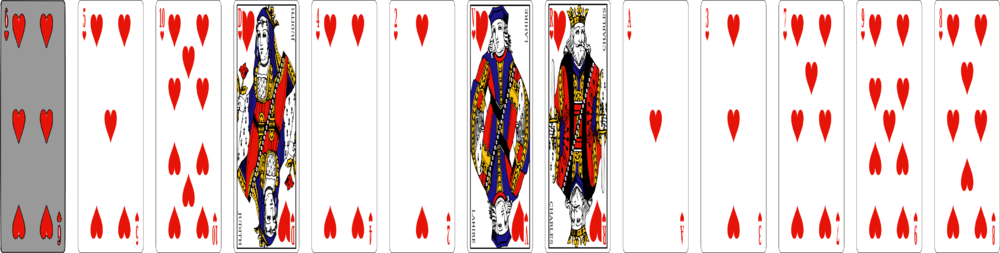
\includegraphics[width=10cm]{ressources/insertion-2.png}
        \captionof{figure}{Replacer la carte dans l'espace}
        \label{pique}
    \end{center}
    \note{la carte est dans le tas trié}
    \hyperlink{menu}{Retour menu}

\end{frame}

\begin{frame}
    \frametitle{Tri par insertion en place}

    \begin{center}
        \centering
        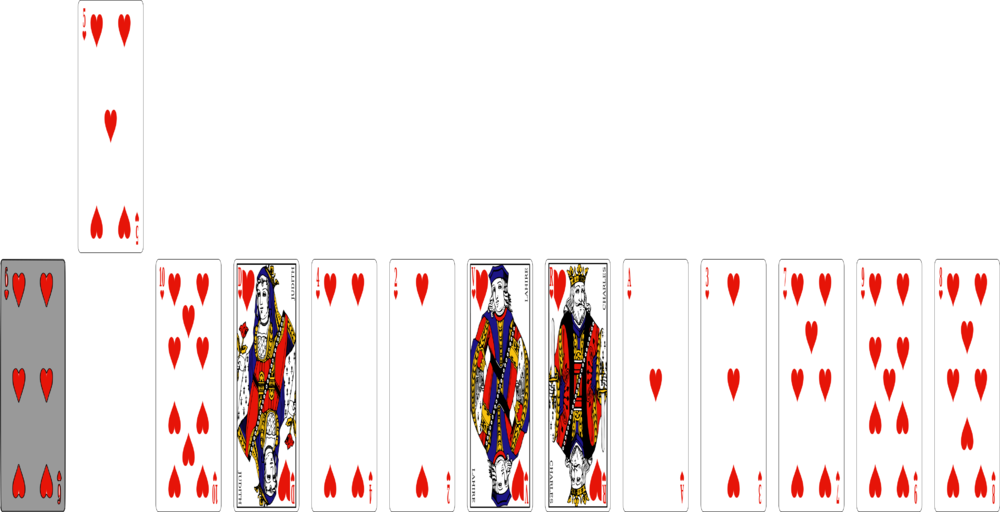
\includegraphics[width=10cm]{ressources/insertion-3.png}
        \captionof{figure}{Mémoriser la première carte dans le tas non trié}
        \label{pique}
    \end{center}
    \note{la carte est dans le tas trié}
    \hyperlink{menu}{Retour menu}

\end{frame}

\begin{frame}
    \frametitle{Tri par insertion en place}

    \begin{center}
        \centering
        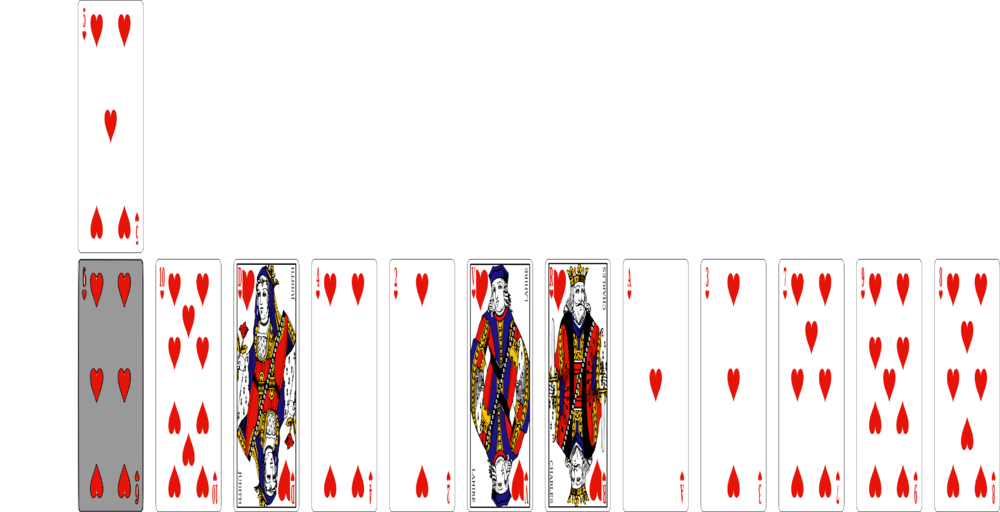
\includegraphics[width=10cm]{ressources/insertion-4.png}
        \captionof{figure}{Décaler les cartes supérieures déjà triées}
        \label{pique}
    \end{center}
    \note{Ici pas de carte triée encore}
    \hyperlink{menu}{Retour menu}

\end{frame}

\begin{frame}
    \frametitle{Tri par insertion en place}

    \begin{center}
        \centering
        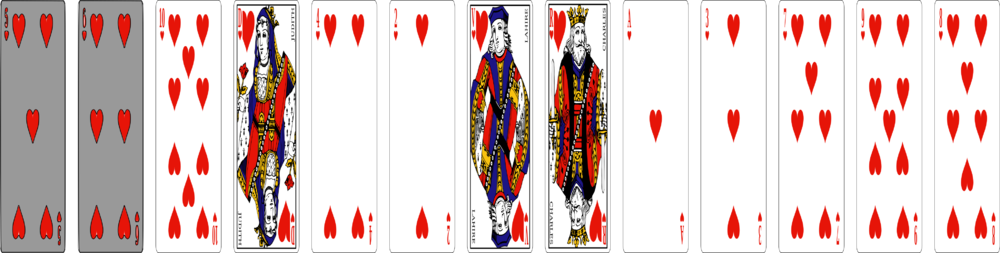
\includegraphics[width=10cm]{ressources/insertion-5.png}
        \captionof{figure}{Replacer la carte dans l'espace}
        \label{pique}
    \end{center}
    \note{la carte est dans le tas trié}
    \hyperlink{menu}{Retour menu}

\end{frame}

\begin{frame}
    \frametitle{Tri par insertion en place}

    \begin{center}
        \centering
        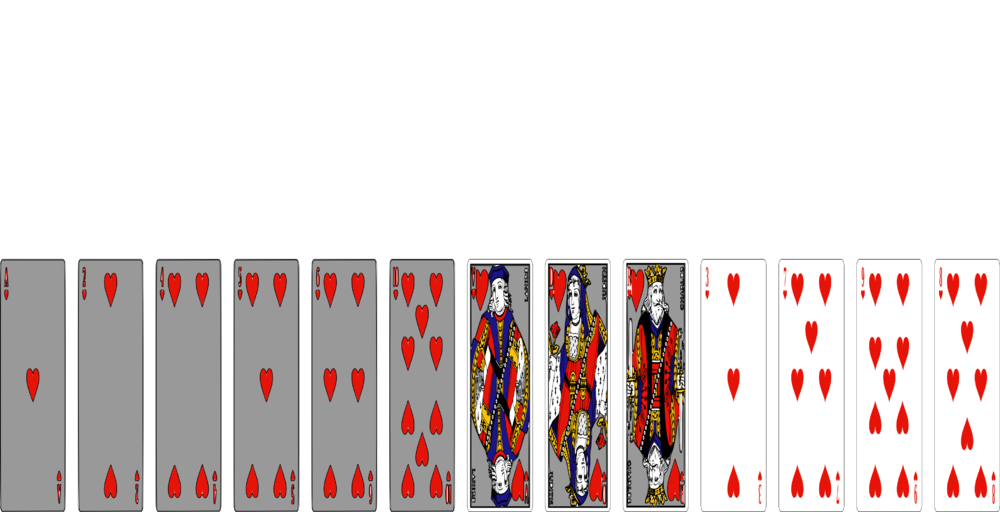
\includegraphics[width=10cm]{ressources/insertion-5-5.png}
        \captionof{figure}{Après plusieurs itérations}
        \label{pique}
    \end{center}
    \hyperlink{menu}{Retour menu}

\end{frame}

\begin{frame}
    \frametitle{Tri par insertion en place}

    \begin{center}
        \centering
        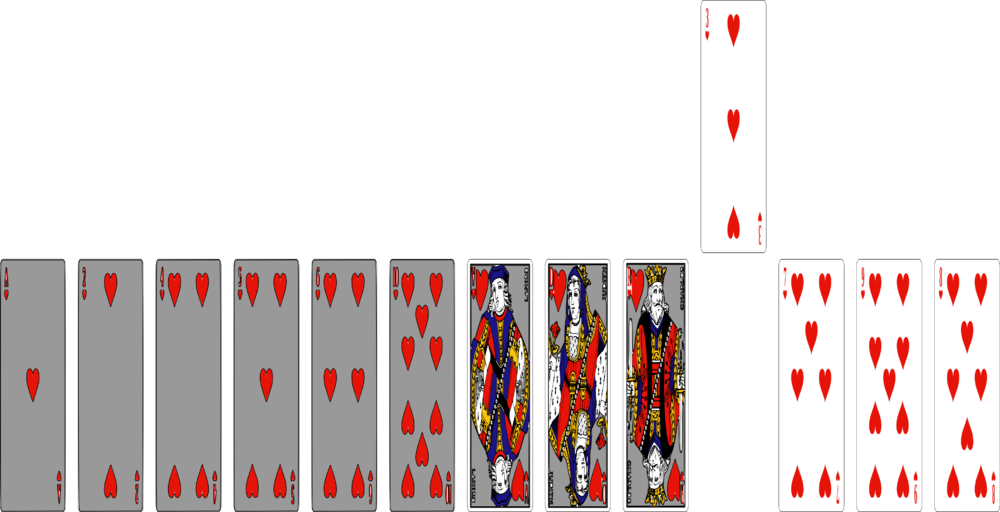
\includegraphics[width=10cm]{ressources/insertion-6.png}
        \captionof{figure}{Mémoriser la première carte dans le tas non trié}
        \label{pique}
    \end{center}
    \note{la carte est dans le tas trié}
    \hyperlink{menu}{Retour menu}

\end{frame}

\begin{frame}
    \frametitle{Tri par insertion en place}

    \begin{center}
        \centering
        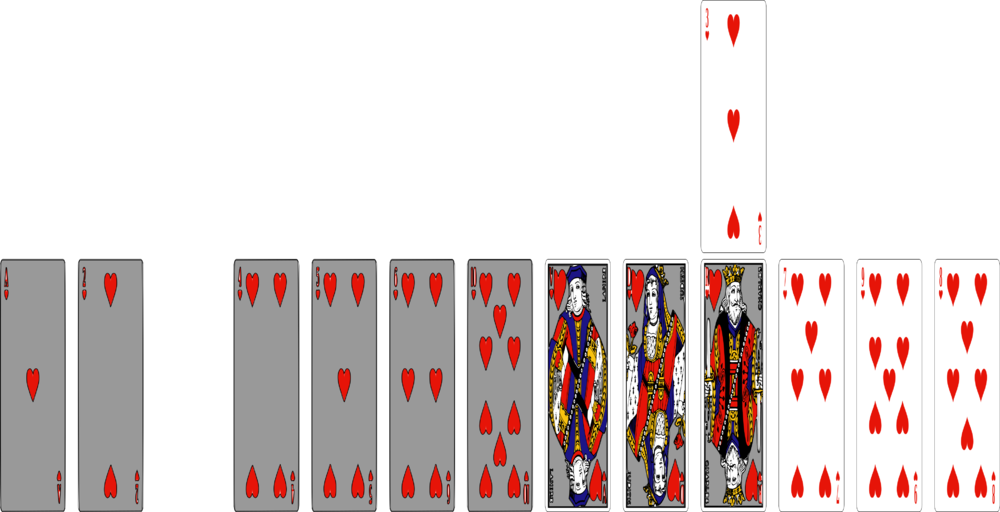
\includegraphics[width=10cm]{ressources/insertion-7.png}
        \captionof{figure}{Décaler les cartes supérieures déjà triées}
        \label{pique}
    \end{center}
    \note{Ici pas de carte triée encore}
    \hyperlink{menu}{Retour menu}

\end{frame}

\begin{frame}
    \frametitle{Tri par insertion en place}

    \begin{center}
        \centering
        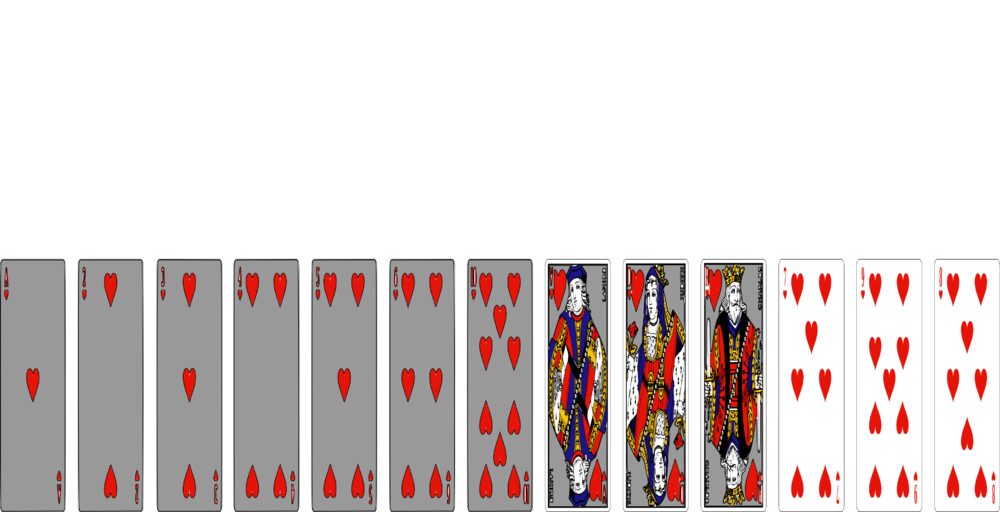
\includegraphics[width=10cm]{ressources/insertion-8.png}
        \captionof{figure}{Insérer la carte dans l'espace}
        \label{pique}
    \end{center}
    \note{la carte est dans le tas trié}
    \hyperlink{menu}{Retour menu}

\end{frame}

\begin{frame}[fragile]
    \frametitle{\hypertarget{insertion2}{Tri par insertion - nouveau tableau}
    }
    \begin{center}
        \begin{lstlisting}[language=bash, basicstyle=\small, xrightmargin=1em]
Pour chaque carte du tas
    Prendre la première carte du tableau non trié.
    Dans le tableau trié, décaler vers la droite toutes les cartes plus grandes.
    Insérer la carte dans le tableau trié.
        \end{lstlisting}
        \captionof{code}{Tri par insertion dans un nouveau tableau}
        \label{CODE}
    \end{center}
\hyperlink{menu}{Retour menu}
\end{frame}
\begin{frame}
    \frametitle{Tri par insertion - nouveau tableau}

    \begin{center}
        \centering
        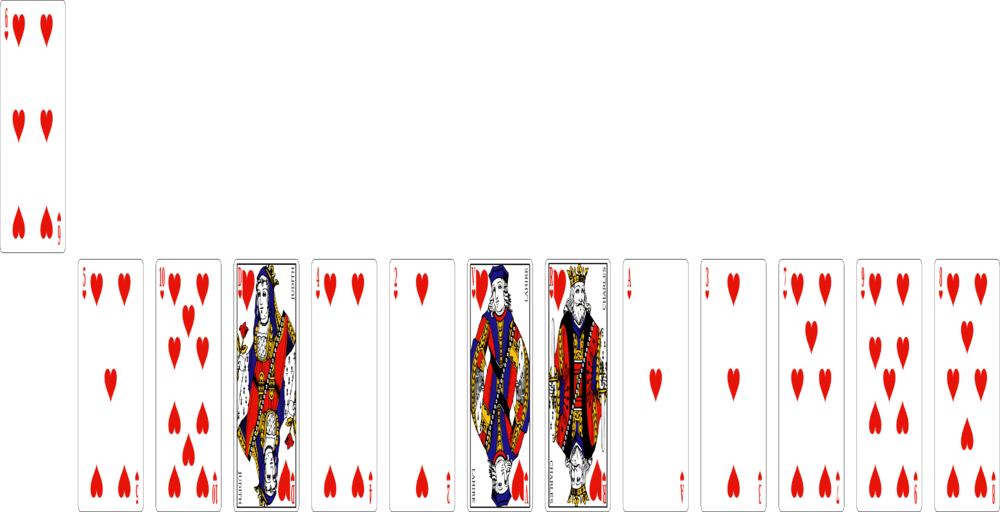
\includegraphics[width=10cm]{ressources/insertion2-1.png}
        \captionof{figure}{Prendre la première carte non triée}
        \label{pique}
    \end{center}
    \hyperlink{menu}{Retour menu}

\end{frame}

\begin{frame}
    \frametitle{Tri par insertion - nouveau tableau}

    \begin{center}
        \centering
        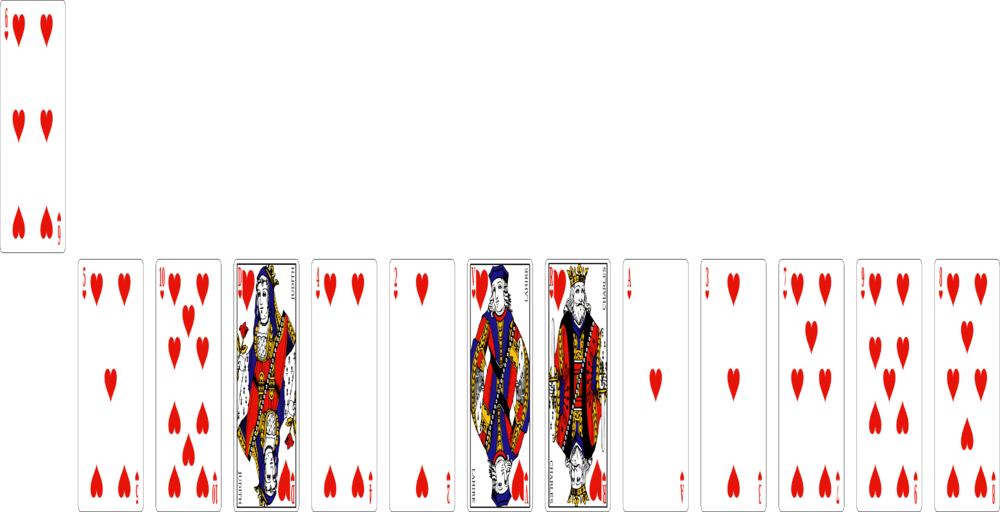
\includegraphics[width=10cm]{ressources/insertion2-1.png}
        \captionof{figure}{Décaler les cartes supérieures du tableau trié}
        \label{pique}
    \end{center}
    \hyperlink{menu}{Retour menu}

\end{frame}

\begin{frame}
    \frametitle{Tri par insertion - nouveau tableau}

    \begin{center}
        \centering
        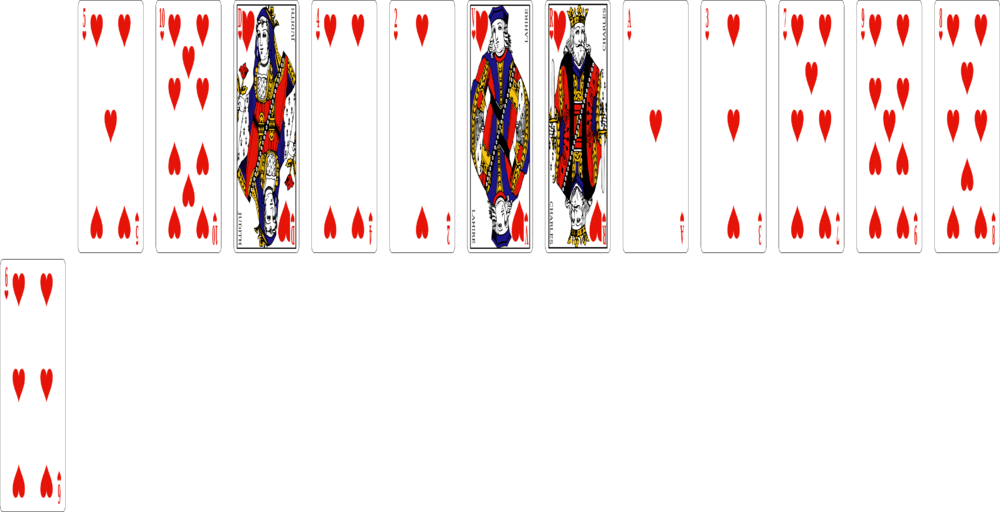
\includegraphics[width=10cm]{ressources/insertion2-2.png}
        \captionof{figure}{Insérer la carte dans le tableau triée}
        \label{pique}
    \end{center}
    \hyperlink{menu}{Retour menu}

\end{frame}


\begin{frame}
    \frametitle{Tri par insertion - nouveau tableau}

    \begin{center}
        \centering
        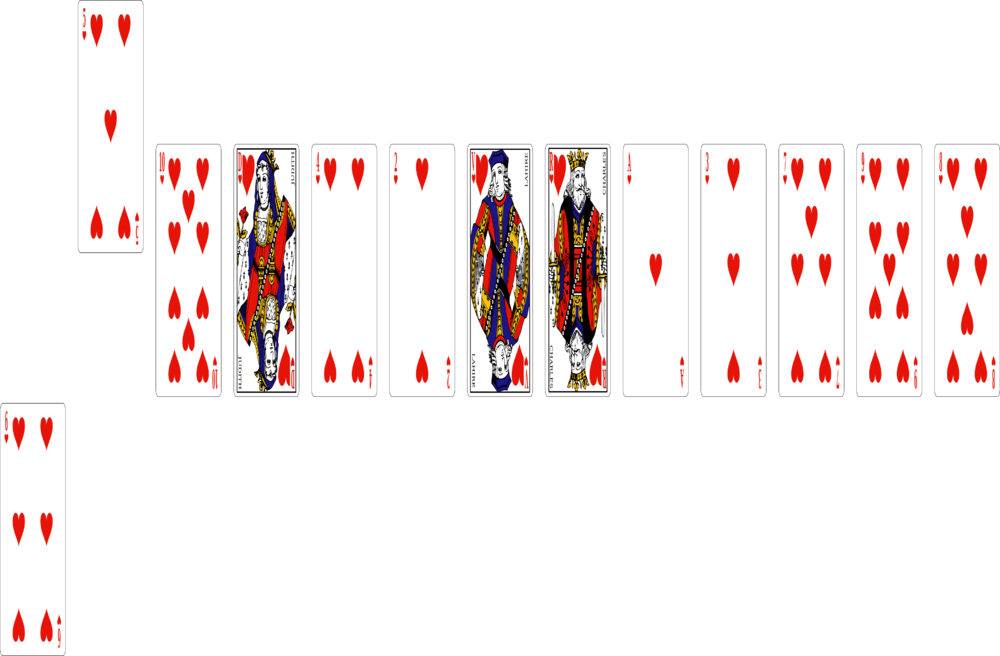
\includegraphics[width=10cm]{ressources/insertion2-3.png}
        \captionof{figure}{Prendre la première carte non triée}
        \label{pique}
    \end{center}
    \hyperlink{menu}{Retour menu}

\end{frame}

\begin{frame}
    \frametitle{Tri par insertion - nouveau tableau}

    \begin{center}
        \centering
        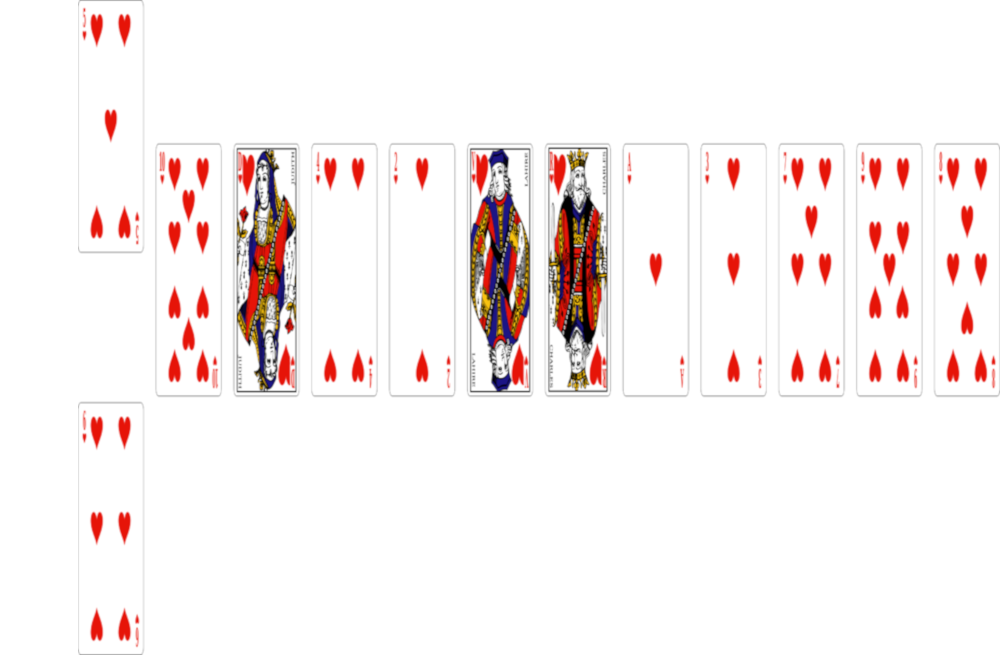
\includegraphics[width=10cm]{ressources/insertion2-4.png}
        \captionof{figure}{Décaler les cartes supérieures du tableau trié}
        \label{pique}
    \end{center}
    \hyperlink{menu}{Retour menu}

\end{frame}

\begin{frame}
    \frametitle{Tri par insertion - nouveau tableau}

    \begin{center}
        \centering
        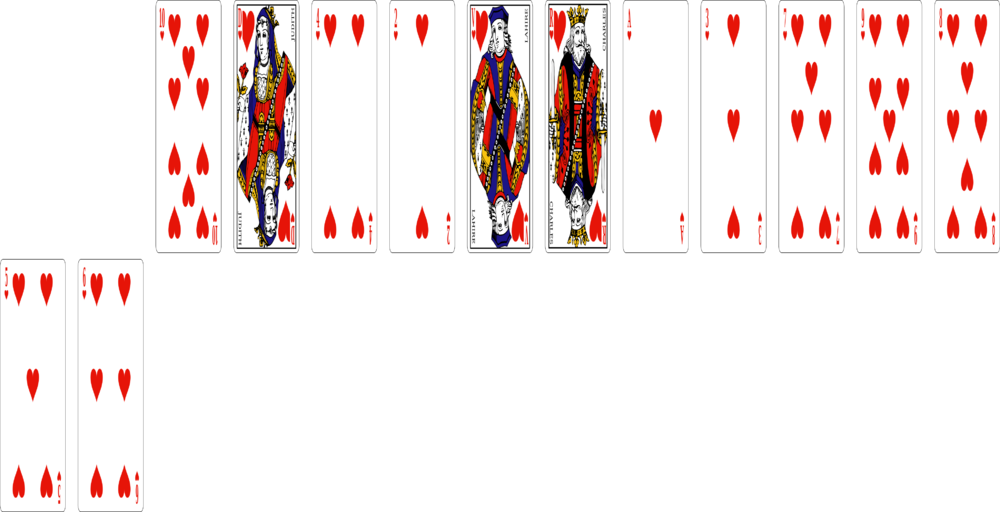
\includegraphics[width=10cm]{ressources/insertion2-5.png}
        \captionof{figure}{Insérer la carte dans le tableau triée}
        \label{pique}
    \end{center}
    \hyperlink{menu}{Retour menu}

\end{frame}

\section{Transposer au tri de données}
\begin{frame}[fragile]
Quand on passe un tableau en argument à une fonction, cette dernière manipule le tableau original.
\begin{center}
\begin{lstlisting}[language=Python]
def ma_fonction(tab: list)->None:
    tab[2] = 199
    
tab = [3, 8, 1, 10, 9]
ma_fonction(tab)
\end{lstlisting}
\end{center}
\begin{center}
\centering
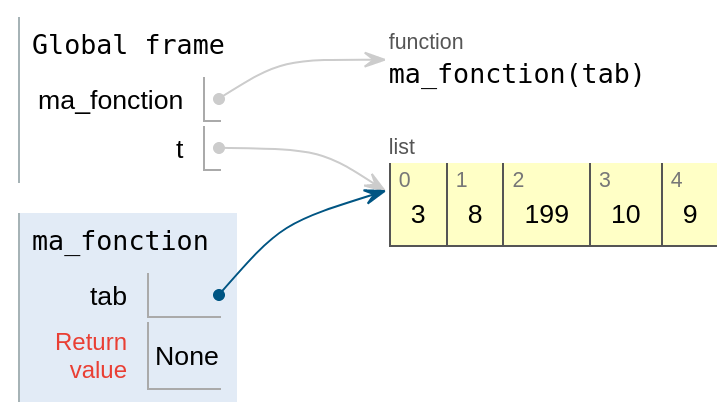
\includegraphics[width=7cm]{ressources/tutor-mutable.png}
\captionof{figure}{La fonction modifie le tableau original}
\label{IMG}
\end{center}
\note[item]{Il faut avoir conscience que les données d'origine sont modifiées. Il ne sert à rien que la fonction renvoie le tableau.}
\note[item]{on va implémenter tri en place; tri dans nouveau tableau dans exercices}
\end{frame}

\subsection{Tri par sélection}
\subsubsection{Implémentation}
\begin{frame}[fragile]
    \frametitle{Rappel de l'algorithme}
    \begin{center}
        \begin{lstlisting}[language=bash, basicstyle=\small,xleftmargin=2em,xrightmargin=2em]
Pour chaque carte du tas
    Trouver la plus petite carte dans la partie non triée.
    Échanger cette carte avec la première de la partie non triée.
\end{lstlisting}
        \captionof{code}{Tri par sélection (en place)}
        \label{CODE}
    \end{center}
\end{frame}
\begin{frame}
    \frametitle{Tri par sélection - question préparatoire}

    \begin{activite}
        \begin{enumerate}
            \item Écrire la fonction \textbf{trouver\_mini(tab: list) $\rightarrow$ int} qui renvoie l'indice du plus petit élément de \emph{tab}.
        \end{enumerate}
    \end{activite}

\end{frame}

\begin{frame}[fragile]
    \frametitle{Correction}

    \begin{center}
    \begin{lstlisting}[language=Python, basicstyle=\small]
def trouver_mini(tab: list)->int:
    """
    Trouve l'indice du plus petit élément
    """
    i_mini = 0
    for j in range(1, len(tab)):
        if tab[j] < tab[i_mini]:
            i_mini = j
    return i_mini
\end{lstlisting}
    \end{center}

\end{frame}
\begin{frame}
    \frametitle{Tri par sélection - Implémentation}
    \setcounter{compteuractivite}{1}
    \begin{activite}        
        \begin{enumerate}
            \setcounter{enumi}{1}
            \item Adapter la fonction précédente pour renvoyer l'indice du plus petit élément de \emph{tab}, compris entre l'indice \emph{i\_depart} et la fin du tableau. La signature de la fonction deviendra \textbf{trouver\_mini(tab: list, i\_depart: int) $\rightarrow$ int}.
            \item Écrire la fonction \textbf{echanger(tab: list, i: int, j: int) $\rightarrow$ None} qui échange les éléments d'indice \emph{i} et \emph{j} du tableau \emph{tab}.
            \item Écrire la fonction \textbf{tri\_selection(tab: list) $\rightarrow$ None} qui effectue un tri par sélection sur \emph{tab}.
        \end{enumerate}
    \end{activite}

\end{frame}

\begin{frame}
    \frametitle{Correction}

    \lstinputlisting[firstline=19 ,lastline=28, basicstyle=\small, xrightmargin=1em ]{"scripts/tri-selection.py"}

\end{frame}

\begin{frame}
    \frametitle{Correction}

    \lstinputlisting[firstline=12 ,lastline=16, basicstyle=\small, xrightmargin=1em  ]{"scripts/tri-selection.py"}

\end{frame}

\begin{frame}
    \frametitle{Correction}

    \lstinputlisting[firstline=31 ,lastline=37,basicstyle=\small, xrightmargin=1em  ]{"scripts/tri-selection.py"}

\end{frame}

\begin{frame}
    \frametitle{Tri par sélection - Tester}
    \setcounter{compteuractivite}{1}
    \begin{activite}
        \begin{enumerate}
            \setcounter{enumi}{4}
            \item Construire par compréhension un tableau des entiers de 1 à 13.
            \item Mélanger le tableau à l'aide de la méthode \emph{shuffle} de la bibliothèque \emph{random}.
            \item Trier le tableau à l'aide de la fonction \emph{tri\_selection}.
        \end{enumerate}
    \end{activite}

\end{frame}

\begin{frame}
    \frametitle{Correction}

    \lstinputlisting[firstline=40 ,lastline=42,basicstyle=\small, xrightmargin=1em  ]{"scripts/tri-selection.py"}

\end{frame}
\subsubsection{Terminaison}
\begin{frame}
    \frametitle{Preuve de terminaison: variant de boucle}

    La terminaison de la fonction est triviale. Le tri est composé de deux boucles bornées donc qui terminent.

\end{frame}

\subsubsection{Correction}
\begin{frame}
    \frametitle{Preuve de correction: invariant de boucle}

    Avant chaque itération de la boucle externe, la partie gauche du tableau est triée.

    \begin{center}
    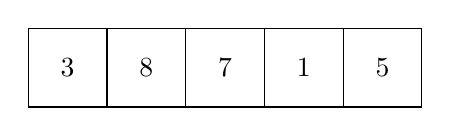
\begin{tikzpicture}
        \draw (0,0) grid (5,1);
        \node at(0.5,0.5) {3};
        \node at(1.5,0.5) {8};
        \node at(2.5,0.5) {7};
        \node at(3.5,0.5) {1};
        \node at(4.5,0.5) {5};

    \end{tikzpicture}
    \captionof{code}{Avant la première itération, la partie gauche est vide, donc triée.}
    \label{CODE}
    \end{center}
\end{frame}

\begin{frame}
    \frametitle{Preuve de correction: invariant de boucle}

    \begin{center}
    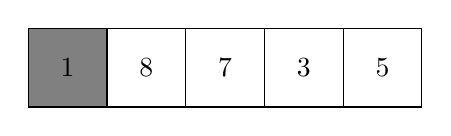
\begin{tikzpicture}
        \fill[gray] (0,0) -- (1,0) -- (1,1) -- (0,1)-- cycle;
        \draw (0,0) grid (5,1);
        \node at(0.5,0.5) {1};
        \node at(1.5,0.5) {8};
        \node at(2.5,0.5) {7};
        \node at(3.5,0.5) {3};
        \node at(4.5,0.5) {5};

    \end{tikzpicture}
    \captionof{code}{Avant la deuxième itération, la partie gauche est triée.}
    \label{CODE}
    \end{center}
\end{frame}

\begin{frame}
    \frametitle{Preuve de correction: invariant de boucle}

    \begin{center}
    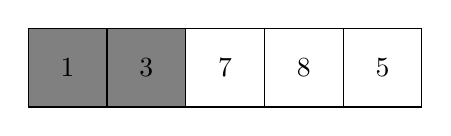
\begin{tikzpicture}        
        \fill[gray] (0,0) -- (2,0) -- (2,1) -- (0,1)-- cycle;
        \draw (0,0) grid (5,1);
        \node at(0.5,0.5) {1};
        \node at(1.5,0.5) {3};
        \node at(2.5,0.5) {7};
        \node at(3.5,0.5) {8};
        \node at(4.5,0.5) {5};

    \end{tikzpicture}
    \captionof{code}{Avant la troisième itération, la partie gauche est triée.}
    \label{CODE}
    \end{center}
\end{frame}

\subsubsection{Complexité}
\begin{frame}[fragile]
    \frametitle{Efficacité du tri}
    \begin{center}
        La boucle externe effectue \textbf{n itérations}.
    \end{center}
    \begin{itemize}
        \item à la première itération de \emph{i}, la boucle de la fonction \emph{trouver\_mini} effectue \emph{n-1} itérations.
        \begin{center}
            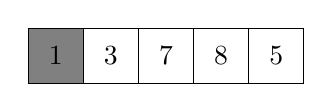
\begin{tikzpicture}[scale=0.7]        
                \fill[gray] (0,0) -- (1,0) -- (1,1) -- (0,1)-- cycle;
                \draw (0,0) grid (5,1);
                \node at(0.5,0.5) {1};
                \node at(1.5,0.5) {3};
                \node at(2.5,0.5) {7};
                \node at(3.5,0.5) {8};
                \node at(4.5,0.5) {5};
        
            \end{tikzpicture}
            \end{center}
        \item à la deuxième itération de \emph{i}, la boucle de la fonction \emph{trouver\_mini} effectue \emph{n-2} itérations.
        \begin{center}
            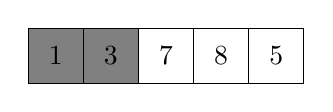
\begin{tikzpicture}[scale=0.7]        
                \fill[gray] (0,0) -- (2,0) -- (2,1) -- (0,1)-- cycle;
                \draw (0,0) grid (5,1);
                \node at(0.5,0.5) {1};
                \node at(1.5,0.5) {3};
                \node at(2.5,0.5) {7};
                \node at(3.5,0.5) {8};
                \node at(4.5,0.5) {5};
        
            \end{tikzpicture}
            \end{center}
        \item \dots
    \end{itemize}
    
\end{frame}

\begin{frame}
    \frametitle{}
    $$\sum_{k=1}^{n-1}{k}=(n-1)+(n-2)+\dots+2+1=\dfrac{n.(n-1)}{2}$$
    \note{démo 2 colonnes inversées de 1+2+...+n-1}
    \begin{aretenir}[]
        Le tri par sélection effectue $\dfrac{n.(n-1)}{2}$ opérations pour ordonner le tableau. 
        
        \centering Le nombre d'opérations dépend de $n^2$.
    \end{aretenir}

\end{frame}

\begin{frame}
    \frametitle{Évolution du nombre d'itérations}

    \begin{center}
    \centering
    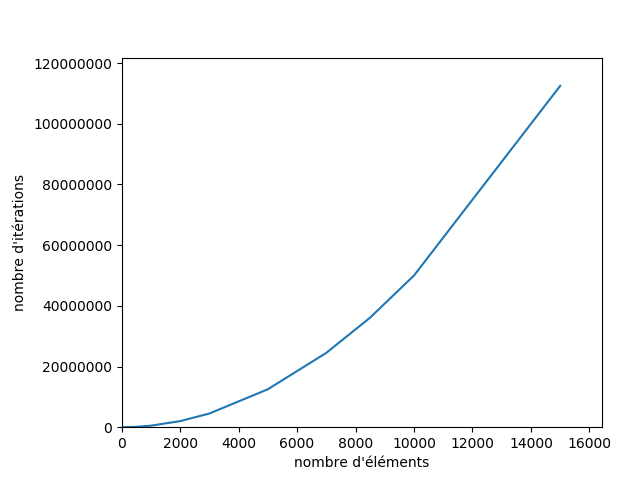
\includegraphics[width=10cm]{ressources/complexite-selection.png}
    \end{center}
\note{15000 éléments $\rightarrow$ 100 millions d'itérations}
\end{frame}
\subsection{Tri par insertion}
\subsubsection{Implémentation}
\begin{frame}
    \frametitle{Tri par insertion}

    \begin{activite}
        \begin{enumerate}
            \item Écrire la fonction \textbf{tri\_insertion(tab: list) $\rightarrow$None} en s'appuyant sur l'algorithme. Les indications suivantes permettront de construire les trois étapes:
                  \begin{itemize}
                      \item \underline{Mémoriser:} définir une variable \emph{en\_cours}, élément en cours de placement et \emph{pos}, position actuelle de cet élément.
                      \item \underline{Décaler:} utiliser une boucle non bornée pour décaler les éléments vers la droite.
                      \item \underline{Insérer:} placer l'élément \emph{en\_cours} à la nouvelle position \emph{pos}.
                  \end{itemize}
            \item Tester la fonction sur un tableau.
        \end{enumerate}
    \end{activite}

\end{frame}

\begin{frame}[fragile]
    \frametitle{Rappel de l'algorithme}

    \begin{center}
        \begin{lstlisting}[language=bash, basicstyle=\small, xrightmargin=1em]
Pour chaque carte du tas
    Mémoriser la carte en cours
    Décaler vers la droite toutes les cartes précédentes, supérieures à la carte en cours.
    Insérer la carte en cours dans l'espace vide.
\end{lstlisting}
        \captionof{code}{Tri par insertion (en place)}
        \label{CODE}
    \end{center}

\end{frame}
\begin{frame}
    \frametitle{Subtilité sur le tableau Python}

    \begin{center}
        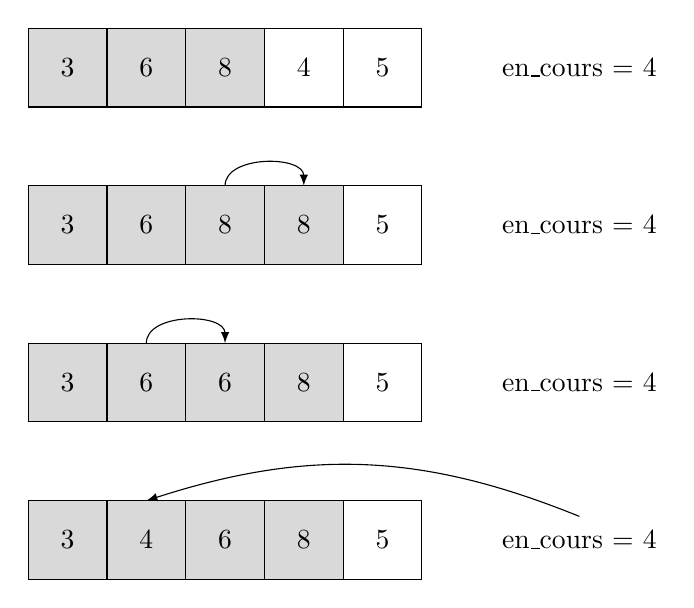
\begin{tikzpicture}
            \fill[gray!30] (0,0) -- (3,0) -- (3,1) -- (0,1)-- cycle;
            \draw (0,0) grid (5,1);
            \node at(0.5,0.5) {3};
            \node at(1.5,0.5) {6};
            \node at(2.5,0.5) {8};
            \node at(3.5,0.5) {4};
            \node at(4.5,0.5) {5};
            \node at(7, 0.5) {en\_cours = 4};
    
            \fill[gray!30] (0,-2) -- (4,-2) -- (4,-1) -- (0,-1)-- cycle;
            \draw (0,-2) grid (5,-1);
            \node at(0.5,-1.5) {3};
            \node at(1.5,-1.5) {6};
            \node at(2.5,-1.5) {8};
            \node at(3.5,-1.5) {8};
            \node at(4.5,-1.5) {5};
            \node at(7, -1.5) {en\_cours = 4};
            \draw[->,>=latex] (2.5,-1) to[bend left=90] (3.5,-1);

            \fill[gray!30] (0,-4) -- (4,-4) -- (4,-3) -- (0,-3)-- cycle;
            \draw (0,-4) grid (5,-3);
            \node at(0.5,-3.5) {3};
            \node at(1.5,-3.5) {6};
            \node at(2.5,-3.5) {6};
            \node at(3.5,-3.5) {8};
            \node at(4.5,-3.5) {5};
            \node at(7, -3.5) {en\_cours = 4};
            \draw[->,>=latex] (1.5,-3) to[bend left=90] (2.5,-3);

            \fill[gray!30] (0,-6) -- (4,-6) -- (4,-5) -- (0,-5)-- cycle;
            \draw (0,-6) grid (5,-5);
            \node at(0.5,-5.5) {3};
            \node at(1.5,-5.5) {4};
            \node at(2.5,-5.5) {6};
            \node at(3.5,-5.5) {8};
            \node at(4.5,-5.5) {5};
            \node at(7, -5.5) {en\_cours = 4};
            \draw[->,>=latex] (7,-5.2) to[bend left=-20] (1.5,-5);
        \end{tikzpicture}
        \captionof{code}{Ce qu'il se passe réellement dans le tableau Python}
        \label{CODE}
        \end{center}

\end{frame}
\begin{frame}
    \frametitle{Correction: boucle principale}

    \lstinputlisting[firstline=12 ,lastline=16, basicstyle=\small, xrightmargin=1em ]{"scripts/tri-insertion.py"}

\end{frame}
\begin{frame}
    \frametitle{Correction: mémoriser}

    \lstinputlisting[firstline=18 ,lastline=19, basicstyle=\small, xrightmargin=1em ]{"scripts/tri-insertion.py"}

\end{frame}

\begin{frame}
    \frametitle{Correction: décaler}

    \lstinputlisting[firstline=21 ,lastline=23, basicstyle=\small, xrightmargin=1em ]{"scripts/tri-insertion.py"}

\end{frame} 
\begin{frame}
    \frametitle{Correction: insérer}

    \lstinputlisting[firstline=25 ,lastline=25, basicstyle=\small, xrightmargin=1em ]{"scripts/tri-insertion.py"}

\end{frame}

\begin{frame}
    \frametitle{Correction: code complet}

    \lstinputlisting[firstline=12 ,lastline=25, basicstyle=\small, xrightmargin=1em ]{"scripts/tri-insertion.py"}

\end{frame}
\begin{frame}
    \frametitle{Correction: tester}

    \lstinputlisting[firstline=28 ,lastline=30, basicstyle=\small, xrightmargin=1em ]{"scripts/tri-insertion.py"}

\end{frame}
\subsubsection{Preuve de terminaison}
\begin{frame}
    \frametitle{Preuve de terminaison}

    Il faut se focaliser sur la boucle interne, non bornée.
    \begin{activite}
        Déterminer un variant de la boucle, qui prouve la terminaison.
    \end{activite}

\end{frame}

\begin{frame}[fragile]
    \frametitle{Correction}

\begin{center}
\begin{lstlisting}[language=Python, basicstyle=\small, xrightmargin=1em]
while pos > 0 and en_cours < tab[pos-1]:
    tab[pos] = tab[pos-1]
    pos = pos-1
\end{lstlisting}
\end{center}

    \emph{pos} est un variant de la boucle. 
    \note{La boucle externe est bornée donc se termine.}
\end{frame} 

\subsubsection{Preuve de correction}
\begin{frame}
    \frametitle{Preuve de correction}

    Comme pour le tri sélection, avant chaque itération de la boucle externe, la partie gauche du tableau est triée.

    \begin{center}
        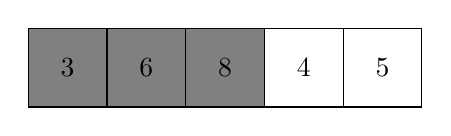
\begin{tikzpicture}
            \fill[gray] (0,0) -- (3,0) -- (3,1) -- (0,1)-- cycle;
            \draw (0,0) grid (5,1);
            \node at(0.5,0.5) {3};
            \node at(1.5,0.5) {6};
            \node at(2.5,0.5) {8};
            \node at(3.5,0.5) {4};
            \node at(4.5,0.5) {5};
    
        \end{tikzpicture}
        \captionof{code}{Insertion de l'élément 4}
        \label{CODE}
        \end{center}

\end{frame}

\begin{frame}
    \frametitle{}

    \begin{center}
        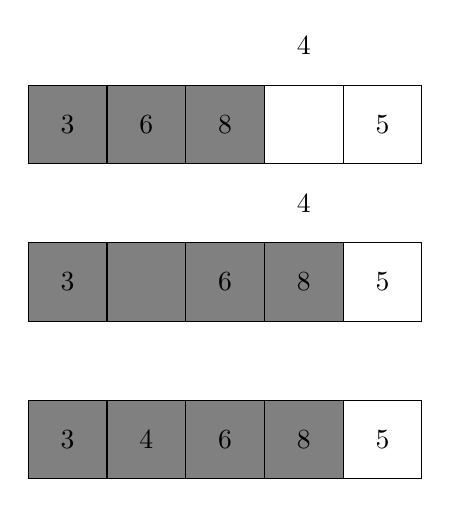
\begin{tikzpicture}
            \fill[gray] (0,0) -- (3,0) -- (3,1) -- (0,1)-- cycle;
            \draw (0,0) grid (5,1);
            \node at(0.5,0.5) {3};
            \node at(1.5,0.5) {6};
            \node at(2.5,0.5) {8};
            \node at(3.5,1.5) {4};
            \node at(4.5,0.5) {5};
    
            \fill[gray] (0,-2) -- (4,-2) -- (4,-1) -- (0,-1)-- cycle;
            \draw (0,-2) grid (5,-1);
            \node at(0.5,-1.5) {3};
            \node at(2.5,-1.5) {6};
            \node at(3.5,-1.5) {8};
            \node at(3.5,-0.5) {4};
            \node at(4.5,-1.5) {5};

            \fill[gray] (0,-4) -- (4,-4) -- (4,-3) -- (0,-3)-- cycle;
            \draw (0,-4) grid (5,-3);
            \node at(0.5,-3.5) {3};
            \node at(2.5,-3.5) {6};
            \node at(3.5,-3.5) {8};
            \node at(1.5,-3.5) {4};
            \node at(4.5,-3.5) {5};
        \end{tikzpicture}
        \captionof{code}{Insertion de l'élément 4}
        \label{CODE}
        \end{center}

\end{frame}
\subsubsection{Complexité}
\begin{frame}[fragile]
    \frametitle{}

    La boucle externe effectue \emph{n} itérations dans tous les cas. 
\begin{center}
\begin{lstlisting}[language=Python, basicstyle=\small, xrightmargin=1em]
for i in range(len(tab)):
\end{lstlisting}
\end{center}
    Cependant, le nombre d'itérations de la boucle interne peut varier.
\begin{center}
\begin{lstlisting}[language=Python, basicstyle=\small, xrightmargin=1em]
while pos > 0 and en_cours < tab[pos-1]:
\end{lstlisting}
\end{center}
    \begin{center}
        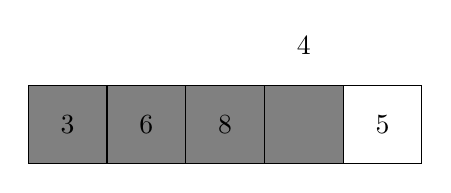
\begin{tikzpicture}    
            \fill[gray] (0,-2) -- (4,-2) -- (4,-1) -- (0,-1)-- cycle;
            \draw (0,-2) grid (5,-1);
            \node at(0.5,-1.5) {3};
            \node at(1.5,-1.5) {6};
            \node at(2.5,-1.5) {8};
            \node at(3.5,-0.5) {4};
            \node at(4.5,-1.5) {5};
        \end{tikzpicture}
        \captionof{code}{Insertion de l'élément 4}
        \label{CODE}
        \end{center}
\end{frame}

\begin{frame}
    \frametitle{}

    \begin{activite}
        \begin{enumerate}
            \item Compter le nombre d'itérations de la boucle interne si le tableau est déjà trié.
            \item Compter le nombre d'itérations de la boucle interne si le tableau est trié dans l'ordre décroissant.
        \end{enumerate}
    \end{activite}

\end{frame}

\begin{frame}[fragile]
    \frametitle{Correction}

    \begin{center}
        \begin{lstlisting}[language=Python, basicstyle=\small, xrightmargin=1em]
while pos > 0 and en_cours < tab[pos-1]:
\end{lstlisting}
        \end{center}
    \begin{center}
        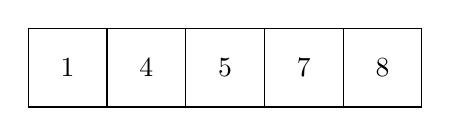
\begin{tikzpicture}  
            \draw (0,-2) grid (5,-1);
            \node at(0.5,-1.5) {1};
            \node at(1.5,-1.5) {4};
            \node at(2.5,-1.5) {5};
            \node at(3.5,-1.5) {7};
            \node at(4.5,-1.5) {8};
        \end{tikzpicture}
        \captionof{code}{Le tableau est déjà trié. La boucle interne n'effectue aucune itération.}
        \label{CODE}
        \end{center}

\end{frame}

\begin{frame}[fragile]
    \frametitle{Correction}

\begin{center}
\begin{lstlisting}[language=Python, basicstyle=\small, xrightmargin=1em]
for i in range(len(tab)):
    en_cours = tab[i]
    pos = i
    while pos > 0 and en_cours < tab[pos-1]:
\end{lstlisting}
\end{center}
    \begin{center}
        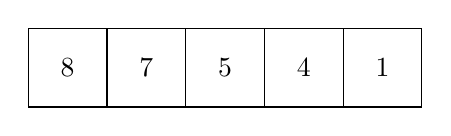
\begin{tikzpicture} 
            \draw (0,-2) grid (5,-1);
            \node at(0.5,-1.5) {8};
            \node at(1.5,-1.5) {7};
            \node at(2.5,-1.5) {5};
            \node at(3.5,-1.5) {4};
            \node at(4.5,-1.5) {1};
        \end{tikzpicture}
        \captionof{code}{Le tableau est inversé. La boucle interne effectue \emph{i} itérations.}
        \label{CODE}
        \end{center}

\end{frame}
\begin{frame}
    \frametitle{}

    \begin{aretenir}[]
        Le tri par insertion effectue un nombre moyen d'opérations qui dépend de $n^2$.
    \end{aretenir}
\note{En pratique, tri un peu meilleur que le tri par sélection.}
\end{frame}
%DODO faire bilan sur les efficacités des 2 tris
\end{document}